\documentclass{article}
\usepackage{amsmath}
\usepackage{setspace}

\usepackage{graphicx}
\graphicspath{{images/}}
\usepackage{wrapfig}
\usepackage{comment}
\usepackage{listings}
\usepackage{xcolor}
\usepackage{float}
\usepackage[style=numeric]{biblatex}
\addbibresource{fish.bib}
\usepackage{comment}

\definecolor{codegreen}{rgb}{0,0.6,0}
\definecolor{codegray}{rgb}{0.5,0.5,0.5}
\definecolor{codepurple}{rgb}{0.58,0,0.82}
\definecolor{backcolour}{rgb}{0.95,0.95,0.92}
 
\lstdefinestyle{mystyle}{
    backgroundcolor=\color{backcolour},
    commentstyle=\color{codegreen},
    keywordstyle=\color{magenta},
    numberstyle=\tiny\color{codegray},
    stringstyle=\color{codepurple},
    basicstyle=\fontsize{10}{12}\ttfamily,
    breakatwhitespace=false,
    breaklines=true,
    %breaklines=false,
    captionpos=b,
    keepspaces=true,
    numbers=left,
    numbersep=5pt,
    showspaces=false,
    showstringspaces=false,
    showtabs=false,
    tabsize=2
}
 
\lstset{style=mystyle}

%\usepackage[letter,margin=1.5in]{geometry}
%\addtolength{\rightmargin}{-0.5in}
%\addtolength{\textwidth}{0.5in}
%\addtolength{\oddsidemargin}{-.875in}
%\addtolength{\evensidemargin}{-.875in}
%\addtolength{\textheight}{1.75in}

\makeatletter
\renewcommand\section{\clearpage\newpage\@startsection {section}{1}{\z@}%
	{-3.5ex \@plus -1ex \@minus -.2ex}%
	{2.3ex \@plus.2ex}%
	{\normalfont\Large\bfseries}}
\makeatother

\begin{document}

%==========================================================================
%==========================================================================
% Title pages.

\begin{comment}
\newcommand{\mytitle}{Report for End of Year on Progress on Fish Tracking Software}
\newcommand{\myauthor}{Ari Spraggins}

\newcommand{\myskip}{\vspace{0.5in}}
\newcommand{\layouttitle}[1]{{\bf\large\MakeUppercase{#1}}}
\setlength{\parindent}{0em}
\doublespace
\pagenumbering{roman}
\thispagestyle{empty}

\begin{center}

	\vspace{4in} 
	\layouttitle{\mytitle} \\ by \\ \myauthor
	
	\vspace{1in}
	A Thesis Submitted to the Faculty of \\
	The Wilkes Honors College \\
	in Partial Fulfillment of the Requirements for the Degree of \\
	Bachelor of Science in Liberal Arts and Sciences \\
	with a Concentration in Physics \\ 
	\vspace{1in} 
	Wilkes Honors College of \\
	Florida Atlantic University \\
	Jupiter, Florida \\
	May \number\year

\end{center}

\newpage

%==========================================================================

\vspace{4in}
\begin{center}
	\layouttitle{\mytitle} \\
	by \\
	\myauthor
\end{center}

\singlespace
\vspace{1in}
This thesis was prepared under the direction of the candidate's thesis advisor, Dr. Yaouen Fily, and has been approved by the members of their supervisory committee. It was submitted to the faculty of the Harriet L. Wilkes Honors College and was accepted in partial fulfillment of the requirements for the degree of Bachelor of Science in Liberal Arts and Sciences.

\vspace{1in}
SUPERVISORY COMMITTEE:

\newcommand{\myrule}{\vspace{0.5in}\rule{4in}{0.5pt} \\}

\myrule
Dr. Yaouen Fily 

\myrule 
{}[second reader]

\myrule
Interim Dean Timothy Steigenga, Harriet L. Wilkes Honors College 

\myrule
Date

\newpage

%==========================================================================

%\begin{center}
%	\layouttitle{Acknowledgements}
%\end{center}
\section*{Acknowledgements}
%\addcontentsline{toc}{section}{Acknowledgements}

\myskip
Some acknowledgements.

\newpage

%==========================================================================

%\begin{center}
%	\layouttitle{Abstract}
%\end{center}
\section*{Abstract}
\addcontentsline{toc}{section}{Abstract}

\myskip
\renewcommand{\arraystretch}{1.5}
\begin{tabular}{@{}l@{\hspace{3ex}}l}
	Author: & \myauthor \\
	Title: & \mytitle \\
	Institution: & Harriet L. Wilkes Honors College, Florida Atlantic University \\
	Thesis Advisor: & Dr. Yaouen Fily \\
	Degree: & Bachelor of Science in Liberal Arts and Sciences \\
	Concentration: & Physics \\
	Year: & \the\year
\end{tabular}

\myskip
\doublespace
\end{comment}
One of the major problem encountered when using the positions of fish in analysis is a tendency for the software to transpose the identities of the two fish whenever they cross. The goal of this program is to analyse that data and to remove that error from it. To do so we are comparing a metric that is unique to the fishes before and after the crossing, in this case a histogram of their brightness, and comparing them.

\singlespace
\newpage

\begin{comment}
%==========================================================================

\tableofcontents

\listoftables

\listoffigures

\newpage

%==========================================================================
\end{comment}

\setlength{\parindent}{1em}
\pagenumbering{arabic}

%==========================================================================
%==========================================================================
% Thesis proper.


\section{Introduction}
\label{introduction}

One of the things that become much easier to track with increases in technology has been tracking the movement of fishes and other similar animals, which has been a boon for the analysis of their movements and behaviors, especially schooling. However, a common issue of automatic tracking is that whenever the position of a fish has been lost, it has no way to regain it's position and track which fish is witch. To solve this issue, we need a way to track the fish from moment to moment. To do this, we are applying two approaches in tandem, both a more naive one that tends to fail in areas where the fish are close together but is computationally light and works well when the fish are far apart; and a second one of comparing a unique identifier for each fish from moment to moment to find the fish with the same identifier which is much more accurate, but computationally intensive, which we got from the paper on the idTracker program from when they tried to tackle the same problem. 

The cavefish trilab on the Jupiter campus(names here?) is currently interested in the evolution of behavior of Mexican Cavefish, which necessitates a lot of video of the fish. To be able to quantify the behavior in a meaningful way, you need automated tracking. Over the last few years the fily group has developed a software to track the fish, but has the issue with the swaps, so this project aims to fix that.

Since the trilab is working with video of cavefish, this presented an opportunity to apply these techniques to clean up the video they have produced.

Before understanding the nature of the problem, we must say a few words about the process. The process starts by picking out the dark spots in the video caused by the contrast between the fish and the light background of the tank.

\begin{figure}[H]
	\centering
	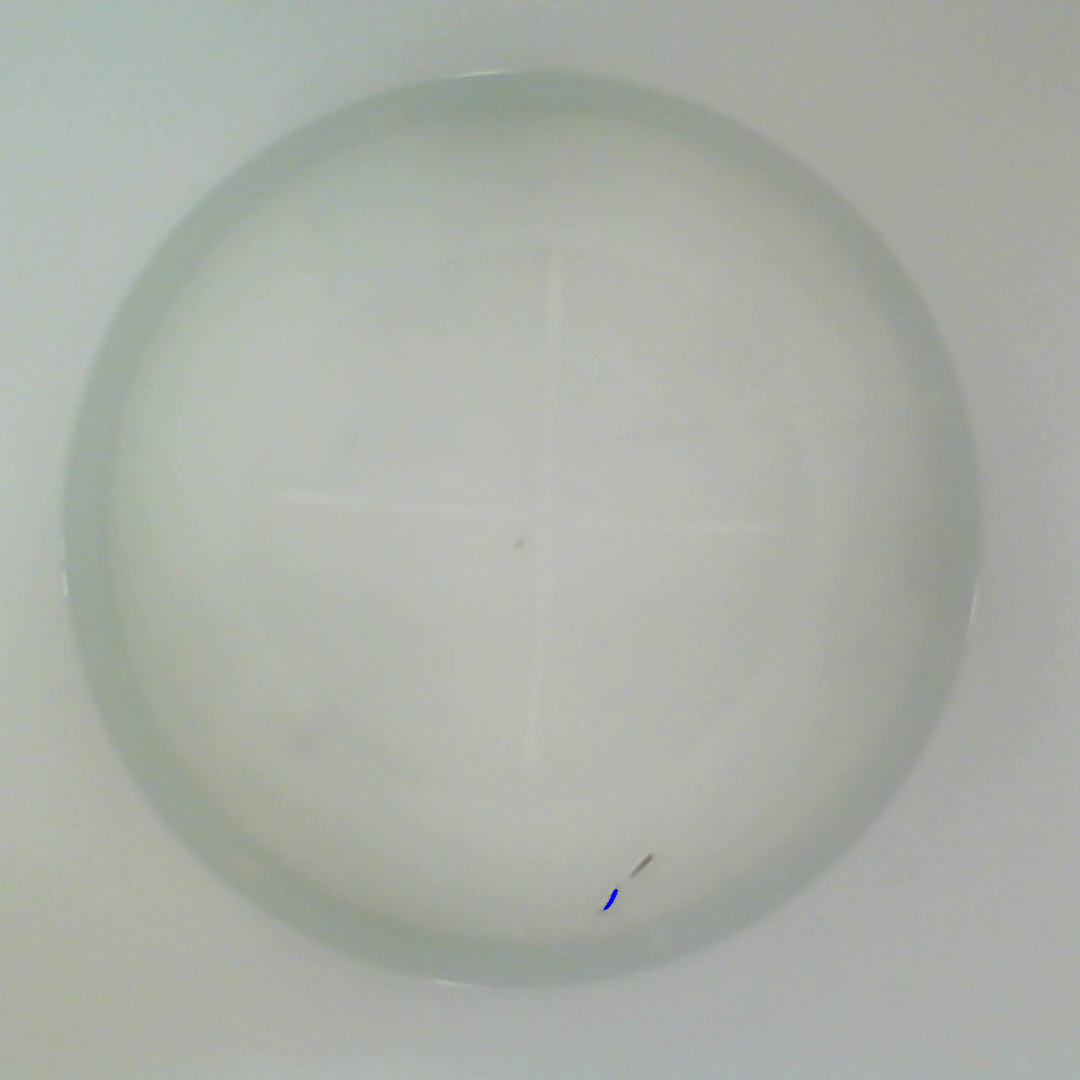
\includegraphics[width=.75\linewidth]{fish}
	\caption{The two fishes}
	\label{fig:fish}
\end{figure}

Once we have the positions of the fish, we can compare how the fish has moved from frame to frame by comparing the distances between their last known positions. If the software swaps the fish, it will look like the fish traveled longer than it should have.
\textbf{\textit{figure of ``distance matrix`` of fishes}}

We can the extend this frame by frame comparison over the regions where the fish are visually distinct. However, in ranges where the positions of the fishes are reported as overlapping, this approach won't work due to the construction of the tracking program. 

\textbf{\textit{Example picture of crossing}}

Instead, during these ranges, we have to take the more involved approach of comparing a visually distinctive feature of the fishes from frame to frame.

\section{Previous work}

The main process by which we are computing the difference between the fish is a process laid in out in the paper on idTracker \cite{idTracker}. The authors of the paper had a similar problem, in that they were having issues with the approach of tracking distances between the fishes position in that the approach both had too much error, and that the error tended to compound in on itself over the length of the tracking process. To combat this, the paper proposed a process by which each fish would be given a unique identifier, which they decided would be the fishes intensity map, which was created by . They then compare the identifiers frame by frame, to determine which fish is witch. We are emulating this process by using a 2d histogram to plot their intensity maps, and using this to compare the frame data.

\section{results}



\subsection{Introduction}
\textbf{\textit{Picture of the fish}}
The basic setup is a tank with two fishes in it and a camera trained on them. 
\textbf{\textit{picture of frame/setup}}

Since we need to track the fish in the setup, we need feed the video captured from this setup to the analysis program. In this case we are using trilab-tracker for this(cite github page) since it has been formulated expressly for this purpose. The trilab-tracker then returns an array for each of the fish containing the pixels and their colors. Once we have the fish saved in a format that we can analyze, the next step is to segment the data into regions based on the number of fish it detects. We do this because the distance based unswapping approach doesn't work on regions where there is only one fish detected, so we need to tell the program where it can use that approach.

\subsection{Distance Based Unswapping}
\textbf{\textit{use current picture 2 here}}
The first approach we tried is taking the positions of the fish and comparing how close they were to their previous positions to check for swaps. This approach works on the regions where there are two fish detected (``nonoverlapping range''), and so we need to confine it to those regions. 

\subsection{Histogram Based Unswapping}
In the overlapping (or regions where one fish is detected), we need an identifier for the fish, so we will use bright spots on fish as identifier. Once we have those identifiers, the easiest way to compare these identifiers is to create histogram of the brightness of the fish. We can then have the program compare the slight differences, because even though look same, they are different enough that the code can pick up the differences. However, one issue that we ran into is that the fish we are using are subpar because they are too uniform in brightness.

\subsection{Accuracy}
\textbf{\textit{show pictures and describe accuracy.}}

One of the first things that I noticed when I compared the results of the unswapping with the manual check was that there was a relatively low accuracy rate. This is probably due to the fish being too uniform, as once we switched to a slightly more accurate fish recognition program, we can expect a slightly more accureate result.

\section{Methods}

One of the things that quickly becomes apparent is that the fish are present as a series of dark pixels against a white background, which means that we can feed the image of a frame to a different software (in this case trilab-tracker) to generate a list of pixels that compose the fishes for tracking. This software returns the fish as either a pair of arrays for the regions where it detects two fish, and a single array where it detects one fish of the form [frame][fish][xpixels, ypixels][color]. Once we have the fish in an array form for ease of operation, we can begin performing an initial unswap by tracking the distance between the fish to determine if there was a swap, by comparing the on and off axis distances of the two possible positions of the fish. The downside of this approach is that it only works in areas in which the tracker returns that there is two fish, so we will first need to determine what regions are overlapping and nonoverlapping. Once we have these nonoverlapping regions, we can begin performing the swap check. 

\begin{minipage}[c]{\textwidth}
\begin{lstlisting}[language=Python]
def swapStatus(pos,i):
    '''
    Detect swaps between consecutive frames based on proximity.
    
    Input:
        pos:Postionts. Array with shape (Nframes,Nfish,Ndimensions),
        i: Frame index. Int.
    
    Output:
        Int. 0 if no swaps, 1 if swapped, 2 if overlapping.
    '''
    nFish=pos.shape[1] #Number of fish
    distanceMatrix=[np.linalg.norm(pos[i+1][0]-pos[i][0]),
                    np.linalg.norm(pos[i+1][1]-pos[i][1]),
                    np.linalg.norm(pos[i+1][0]-pos[i][1]),
                    np.linalg.norm(pos[i+1][1]-pos[i][0])]
    swapCriteron=(distanceMatrix[0]+distanceMatrix[1])-(distanceMatrix[2]+distanceMatrix[3])
    if abs(swapCriteron)<1e-10:
        return 2 #Overlapping
    elif swapCriteron>0:
        return 1 #Swapped
    elif swapCriteron<0:
        return 0 #Normal
    else:
        return -1
\end{lstlisting}
\end{minipage}

Once we have this data for the nonoverlapping ranges, we have to switch approaches for the overlapping regions. Since we can't compare the distances with the software only reporting a single fish, we are forced to use a different technique., we are using the technique of comparing the histograms of the brightness of the fishes before and after an overlapping range, as proposed by the paper on idTracker\cite{idTracker}. The process for this is for us to feed the arrays directly into numpy's histogram2d, which allows us to compute the histograms with a minimal amount of effort other than determining the correct bins. After that we need to manipulate the data slightly so that the histograms are taken as the average over the nonoverlapping regions for more accuracy, and are then saved out for comparison.

\begin{minipage}[c]{\textwidth}
\begin{lstlisting}[language=Python]
for i in tnrange(60,desc='nonOverlappingRange'):
    for k in range(2):
        countSum=0
        countDif=0
        pairData=[]
        for j in range(*nonOverlappingRange[i]):
            fishPixels = fishU[j][k]
            m,l=np.triu_indices(fishPixels.shape[0],k=1)
            d=np.sqrt((fishPixels[l,0]-fishPixels[m,0])**2+(fishPixels[l,1]-fishPixels[m,1])**2)
            bSum=fishPixels[l,2]+fishPixels[m,2]
            bDif=fishPixels[l,2]-fishPixels[m,2]

            heightValuesSum,_,_=np.histogram2d(d,bSum,bins=(binsDist,binsSum))
            histSum+=heightValuesSum
            countSum+=1
            heightValuesDif,_,_=np.histogram2d(d,bDif,bins=(binsDist,binsDif))
            histDif+=heightValuesDif
            countDif+=1
        histSum/=countSum
        histSumList[i,k]=histSum.copy()
        histDif/=countDif
        histDifList[i,k]=histDif.copy()
\end{lstlisting}
\end{minipage}

This produces a histogram, similar to the one seen below. The problem with 

\textbf{\textit{move to results}}

\begin{figure}[H]
	\centering
	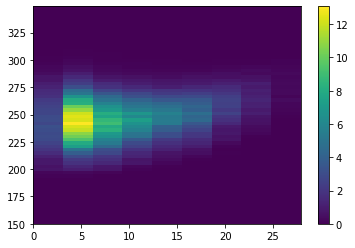
\includegraphics[width=.75\linewidth]{hist}
	\caption{The histogram}
	\label{fig:hist}
\end{figure}


We can then feed this representation into a distance matrix to perform the final check for swaps.

\appendix
\section{An appendix}

%==========================================================================
% Bibliography.

%\printbibliography
%\bibliographystyle{plain}
%\bibliography{fish}


\end{document}
